\documentclass[pdftex]{article}
\usepackage[T1]{fontenc}
\usepackage[utf8]{inputenc}
\usepackage{graphicx}
\usepackage{caption}

\title{PHYS 721 Homework 3}
\author{Nick Tyler}
\date{}


\begin{document}
\maketitle
\begin{enumerate}
	\item The mass of the sum of the four vectors was caculated in the homework assignment last week.
	This graph was fitted with a relatavistic Breit-Wigner distribution.\\
		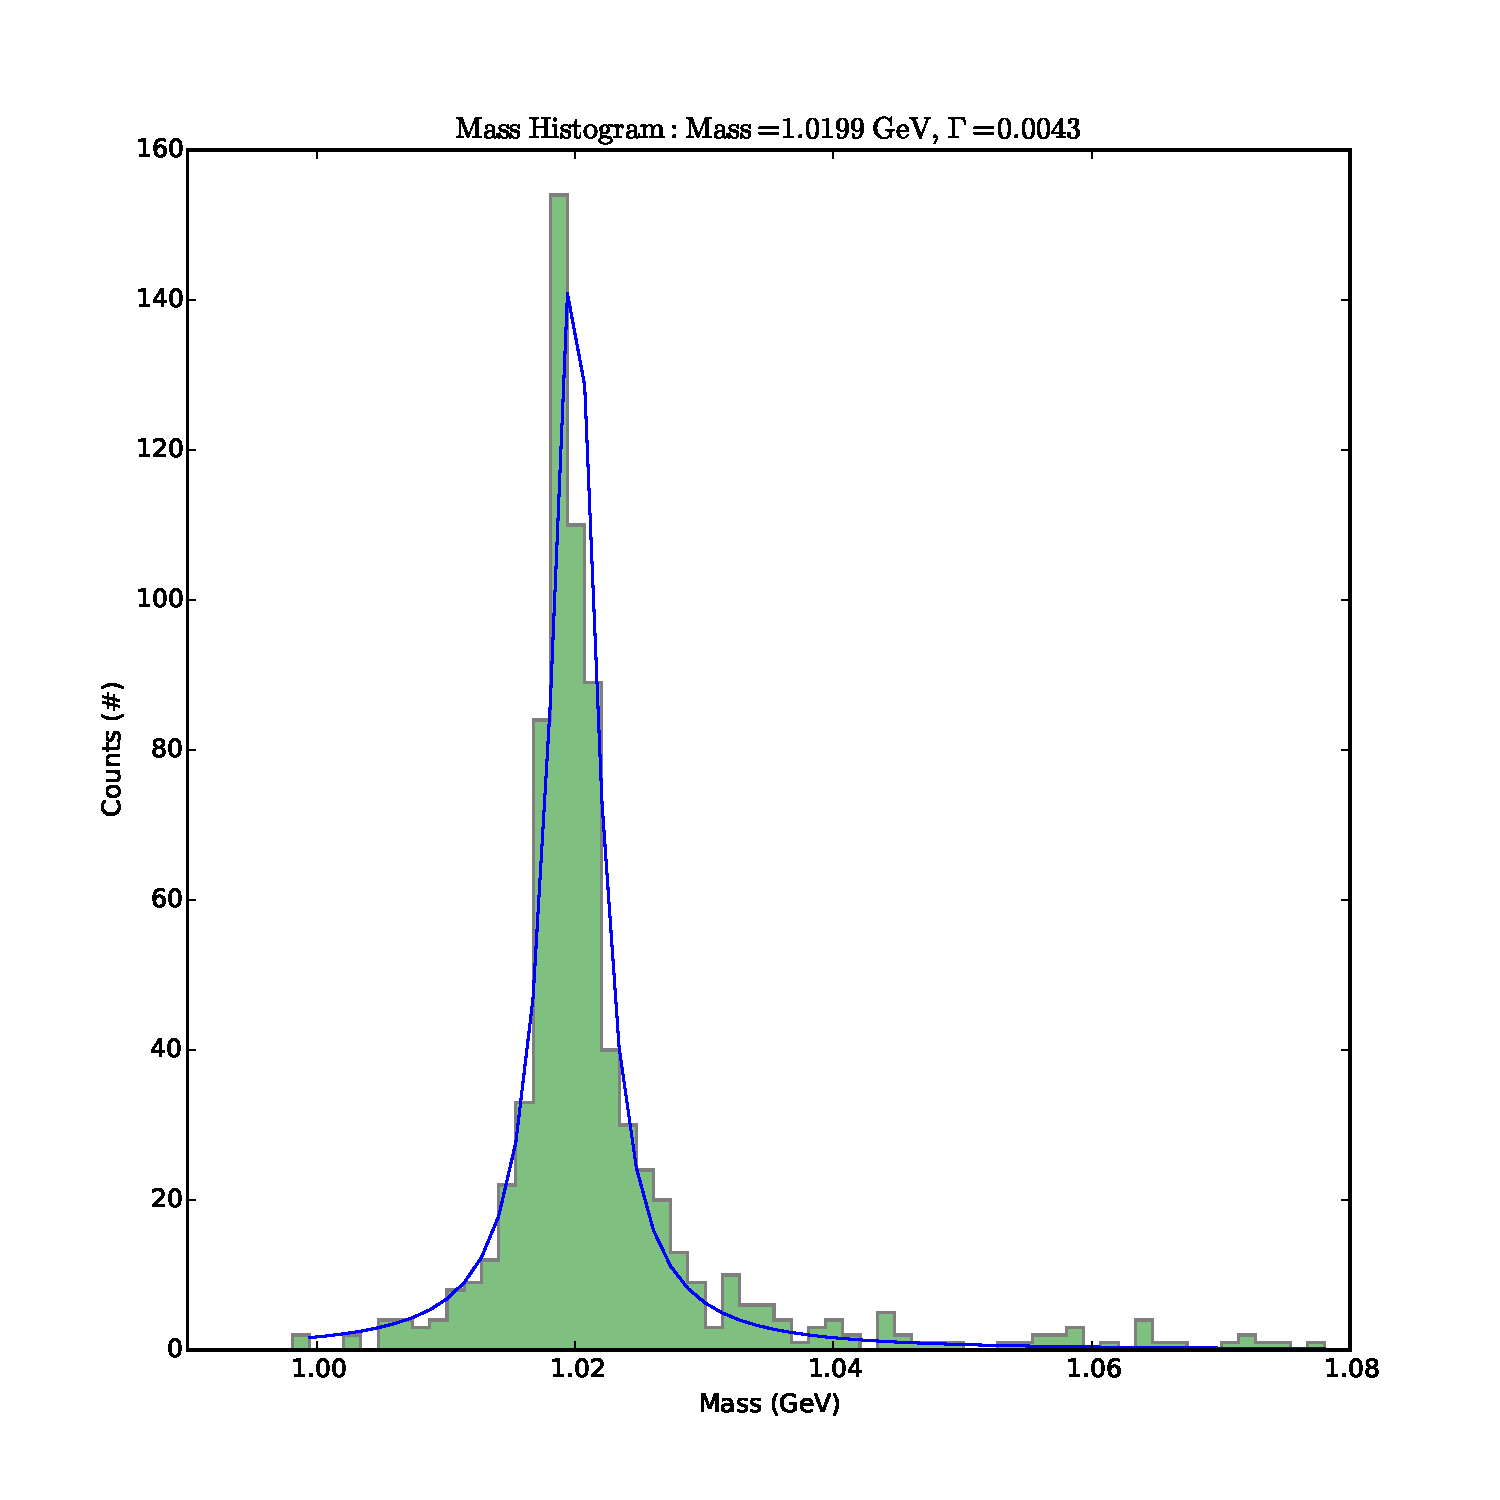
\includegraphics[scale=0.5]{Problem_1.pdf}\\
		\captionof{figure}{Mass Histograms in GeV/$c^2$ with Breit-Wigner fit.}

	\pagebreak
	\item This was also done using ROOTs built in Breit-Wigner distribution.\\
		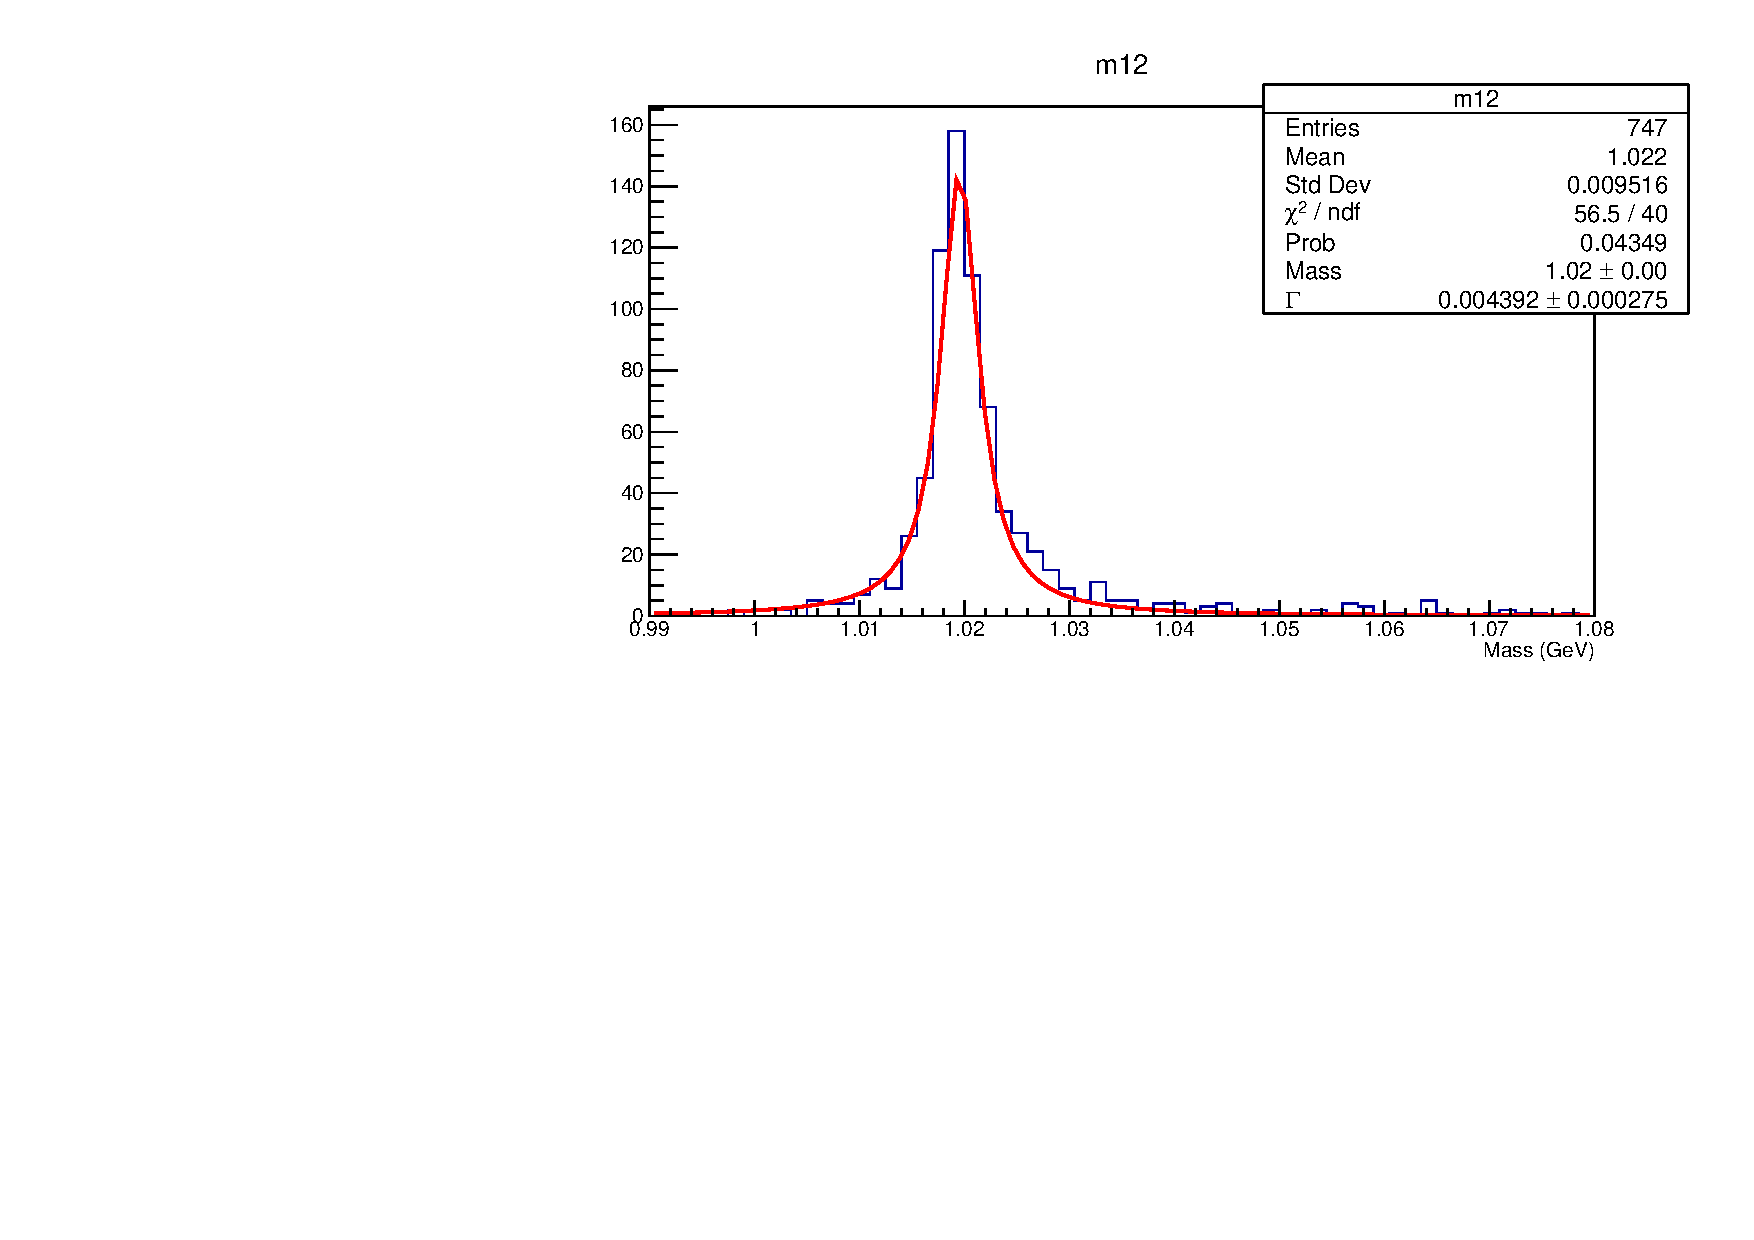
\includegraphics[scale=0.8]{Problem_root_1.pdf}\\
		\captionof{figure}{Mass Histograms in GeV/$c^2$ with Breit-Wigner fit.}

\end{enumerate}

\end{document}